% Options for packages loaded elsewhere
\PassOptionsToPackage{unicode}{hyperref}
\PassOptionsToPackage{hyphens}{url}
\PassOptionsToPackage{dvipsnames,svgnames,x11names}{xcolor}
%
\documentclass[
  letterpaper,
  DIV=11,
  numbers=noendperiod]{scrartcl}

\usepackage{amsmath,amssymb}
\usepackage{iftex}
\ifPDFTeX
  \usepackage[T1]{fontenc}
  \usepackage[utf8]{inputenc}
  \usepackage{textcomp} % provide euro and other symbols
\else % if luatex or xetex
  \usepackage{unicode-math}
  \defaultfontfeatures{Scale=MatchLowercase}
  \defaultfontfeatures[\rmfamily]{Ligatures=TeX,Scale=1}
\fi
\usepackage{lmodern}
\ifPDFTeX\else  
    % xetex/luatex font selection
\fi
% Use upquote if available, for straight quotes in verbatim environments
\IfFileExists{upquote.sty}{\usepackage{upquote}}{}
\IfFileExists{microtype.sty}{% use microtype if available
  \usepackage[]{microtype}
  \UseMicrotypeSet[protrusion]{basicmath} % disable protrusion for tt fonts
}{}
\makeatletter
\@ifundefined{KOMAClassName}{% if non-KOMA class
  \IfFileExists{parskip.sty}{%
    \usepackage{parskip}
  }{% else
    \setlength{\parindent}{0pt}
    \setlength{\parskip}{6pt plus 2pt minus 1pt}}
}{% if KOMA class
  \KOMAoptions{parskip=half}}
\makeatother
\usepackage{xcolor}
\setlength{\emergencystretch}{3em} % prevent overfull lines
\setcounter{secnumdepth}{5}
% Make \paragraph and \subparagraph free-standing
\ifx\paragraph\undefined\else
  \let\oldparagraph\paragraph
  \renewcommand{\paragraph}[1]{\oldparagraph{#1}\mbox{}}
\fi
\ifx\subparagraph\undefined\else
  \let\oldsubparagraph\subparagraph
  \renewcommand{\subparagraph}[1]{\oldsubparagraph{#1}\mbox{}}
\fi


\providecommand{\tightlist}{%
  \setlength{\itemsep}{0pt}\setlength{\parskip}{0pt}}\usepackage{longtable,booktabs,array}
\usepackage{calc} % for calculating minipage widths
% Correct order of tables after \paragraph or \subparagraph
\usepackage{etoolbox}
\makeatletter
\patchcmd\longtable{\par}{\if@noskipsec\mbox{}\fi\par}{}{}
\makeatother
% Allow footnotes in longtable head/foot
\IfFileExists{footnotehyper.sty}{\usepackage{footnotehyper}}{\usepackage{footnote}}
\makesavenoteenv{longtable}
\usepackage{graphicx}
\makeatletter
\def\maxwidth{\ifdim\Gin@nat@width>\linewidth\linewidth\else\Gin@nat@width\fi}
\def\maxheight{\ifdim\Gin@nat@height>\textheight\textheight\else\Gin@nat@height\fi}
\makeatother
% Scale images if necessary, so that they will not overflow the page
% margins by default, and it is still possible to overwrite the defaults
% using explicit options in \includegraphics[width, height, ...]{}
\setkeys{Gin}{width=\maxwidth,height=\maxheight,keepaspectratio}
% Set default figure placement to htbp
\makeatletter
\def\fps@figure{htbp}
\makeatother

\usepackage{booktabs}
\usepackage{longtable}
\usepackage{array}
\usepackage{multirow}
\usepackage{wrapfig}
\usepackage{float}
\usepackage{colortbl}
\usepackage{pdflscape}
\usepackage{tabu}
\usepackage{threeparttable}
\usepackage{threeparttablex}
\usepackage[normalem]{ulem}
\usepackage{makecell}
\usepackage{xcolor}
\KOMAoption{captions}{tableheading}
\makeatletter
\makeatother
\makeatletter
\makeatother
\makeatletter
\@ifpackageloaded{caption}{}{\usepackage{caption}}
\AtBeginDocument{%
\ifdefined\contentsname
  \renewcommand*\contentsname{Table of contents}
\else
  \newcommand\contentsname{Table of contents}
\fi
\ifdefined\listfigurename
  \renewcommand*\listfigurename{List of Figures}
\else
  \newcommand\listfigurename{List of Figures}
\fi
\ifdefined\listtablename
  \renewcommand*\listtablename{List of Tables}
\else
  \newcommand\listtablename{List of Tables}
\fi
\ifdefined\figurename
  \renewcommand*\figurename{Figure}
\else
  \newcommand\figurename{Figure}
\fi
\ifdefined\tablename
  \renewcommand*\tablename{Table}
\else
  \newcommand\tablename{Table}
\fi
}
\@ifpackageloaded{float}{}{\usepackage{float}}
\floatstyle{ruled}
\@ifundefined{c@chapter}{\newfloat{codelisting}{h}{lop}}{\newfloat{codelisting}{h}{lop}[chapter]}
\floatname{codelisting}{Listing}
\newcommand*\listoflistings{\listof{codelisting}{List of Listings}}
\makeatother
\makeatletter
\@ifpackageloaded{caption}{}{\usepackage{caption}}
\@ifpackageloaded{subcaption}{}{\usepackage{subcaption}}
\makeatother
\makeatletter
\@ifpackageloaded{tcolorbox}{}{\usepackage[skins,breakable]{tcolorbox}}
\makeatother
\makeatletter
\@ifundefined{shadecolor}{\definecolor{shadecolor}{rgb}{.97, .97, .97}}
\makeatother
\makeatletter
\makeatother
\makeatletter
\makeatother
\ifLuaTeX
  \usepackage{selnolig}  % disable illegal ligatures
\fi
\IfFileExists{bookmark.sty}{\usepackage{bookmark}}{\usepackage{hyperref}}
\IfFileExists{xurl.sty}{\usepackage{xurl}}{} % add URL line breaks if available
\urlstyle{same} % disable monospaced font for URLs
\hypersetup{
  pdftitle={Indicador de Desarrollo Económico (2018-2023)},
  pdfauthor={Sofia Melcarne, Carlos Gila y Enrique Sayas},
  colorlinks=true,
  linkcolor={blue},
  filecolor={Maroon},
  citecolor={Blue},
  urlcolor={Blue},
  pdfcreator={LaTeX via pandoc}}

\title{Indicador de Desarrollo Económico (2018-2023)}
\author{Sofia Melcarne, Carlos Gila y Enrique Sayas}
\date{}

\begin{document}
\maketitle
\ifdefined\Shaded\renewenvironment{Shaded}{\begin{tcolorbox}[borderline west={3pt}{0pt}{shadecolor}, sharp corners, enhanced, interior hidden, frame hidden, boxrule=0pt, breakable]}{\end{tcolorbox}}\fi

\renewcommand*\contentsname{Table of contents}
{
\hypersetup{linkcolor=}
\setcounter{tocdepth}{3}
\tableofcontents
}
\hypertarget{introducciuxf3n}{%
\section{Introducción}\label{introducciuxf3n}}

\hypertarget{planteamiento-del-problema}{%
\section{Planteamiento del problema}\label{planteamiento-del-problema}}

\hypertarget{descriptivo}{%
\section{Descriptivo}\label{descriptivo}}

El Indicador de Desarrollo Económico (2018-2023) tiene como objetivo
mostrar la distancia de los países de la Unión Europea respecto al peor
caso de desarrollo económico. En este caso, se ha establecido la media
europea como base para el diseño del ranking (EU27 = 100).

Para la elaboración del indicador se ha seleccionado cinco variables
económicas clave:

\begin{itemize}
\tightlist
\item
  Evolución del PIB per Capita deflactado respecto al año 2005.
\item
  Evolución de la tasa de paro
\item
  Evolución de la presión fiscal.
\item
  Evolución del poder adquisitivo de las familias respecto a la media
  europea.
\item
  Evolución de la deuda pública.
\end{itemize}

Para ello, han sido utilizados los últimos datos disponibles en
Eurostat:

\begin{longtable}[]{@{}ll@{}}
\toprule\noalign{}
Datos & Eurostat \\
\midrule\noalign{}
\endhead
\bottomrule\noalign{}
\endlastfoot
PIB & namq\_10\_gdp \\
Población & demo\_pjan \\
Deflactor & namq\_10\_gdp \\
Tasa de Paro & une\_rt\_m \\
Presión Fiscal & gov\_10a\_taxag \\
Poder Aquisitivo de las Familias & tec00114 \\
Deuda Pública & gov\_10dd\_edpt1 \\
\end{longtable}

No todas las variables serán igual de relevantes a la hora de calcular
el indicador. Esto se debe a que en la variable Tasa de Paro se
desconoce el número de fijos discontinuos en España, lo que puede llevar
a una distorsión en la evolución de la tasa de desempleo entre 2018 y
2023.

\hypertarget{pib-per-capita}{%
\subsection{PIB per Capita}\label{pib-per-capita}}

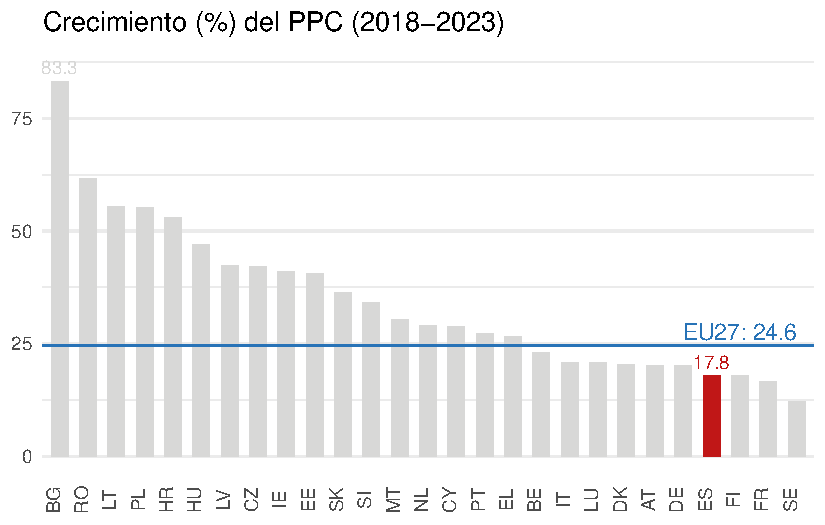
\includegraphics{Trabajo_files/figure-pdf/unnamed-chunk-14-1.pdf}

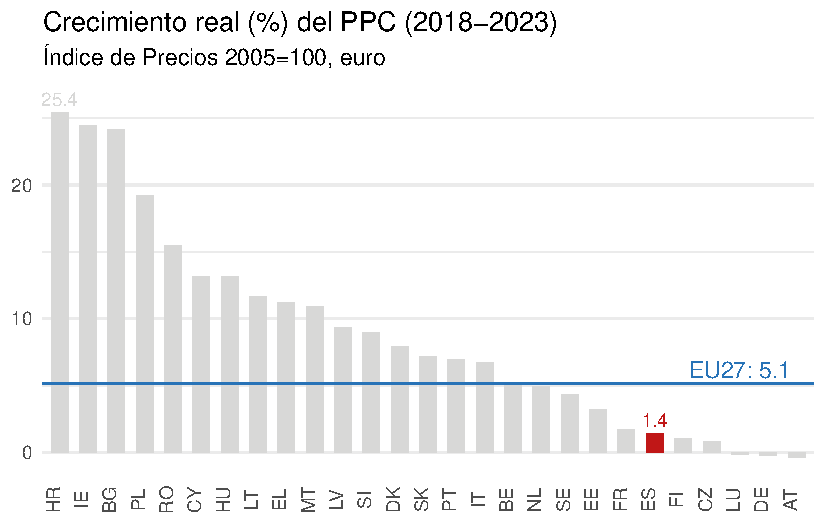
\includegraphics{Trabajo_files/figure-pdf/unnamed-chunk-15-1.pdf}

\hypertarget{tasa-de-paro}{%
\subsection{Tasa de Paro}\label{tasa-de-paro}}

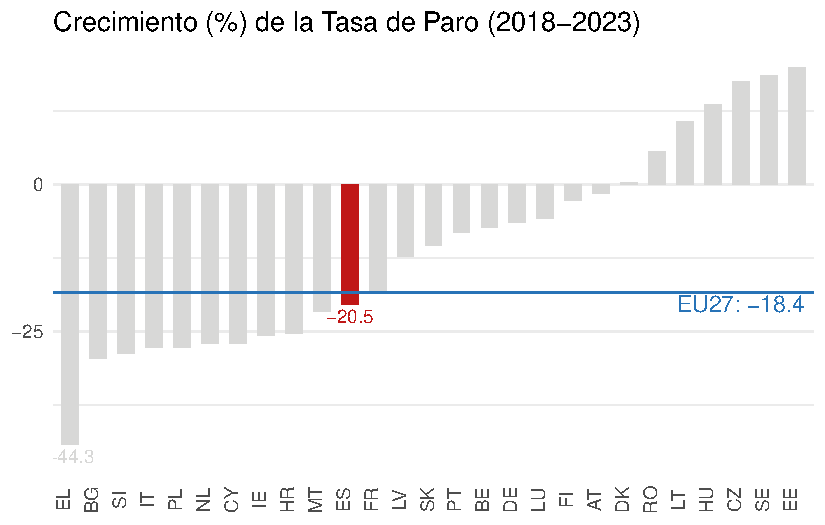
\includegraphics{Trabajo_files/figure-pdf/unnamed-chunk-19-1.pdf}

\hypertarget{presiuxf3n-fiscal}{%
\subsection{Presión Fiscal}\label{presiuxf3n-fiscal}}

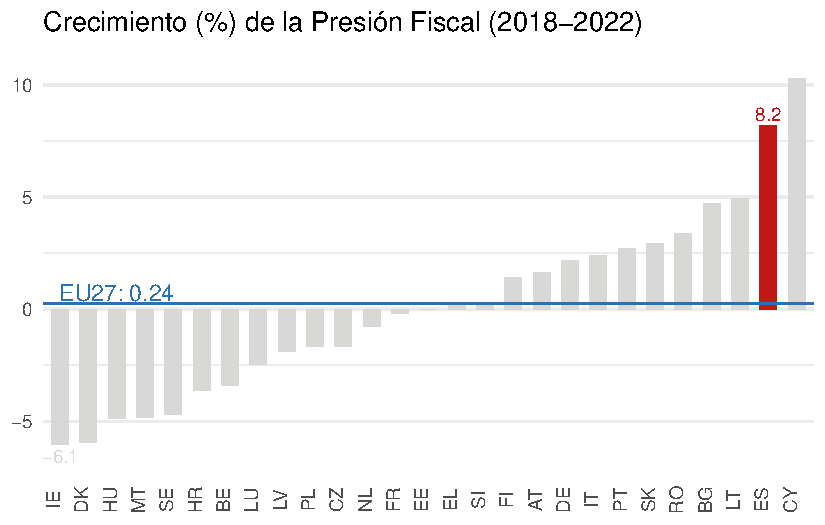
\includegraphics{Trabajo_files/figure-pdf/unnamed-chunk-23-1.pdf}

\hypertarget{evoluciuxf3n-del-poder-adquisitivo-de-las-familias-ppa}{%
\subsection{Evolución del poder adquisitivo de las familias
(PPA)}\label{evoluciuxf3n-del-poder-adquisitivo-de-las-familias-ppa}}

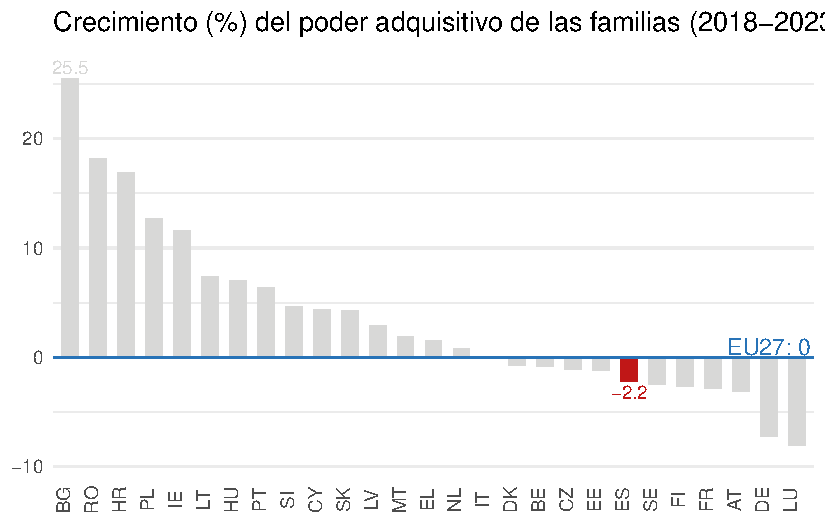
\includegraphics{Trabajo_files/figure-pdf/unnamed-chunk-27-1.pdf}

\hypertarget{deuda-puxfablica}{%
\subsection{Deuda pública}\label{deuda-puxfablica}}

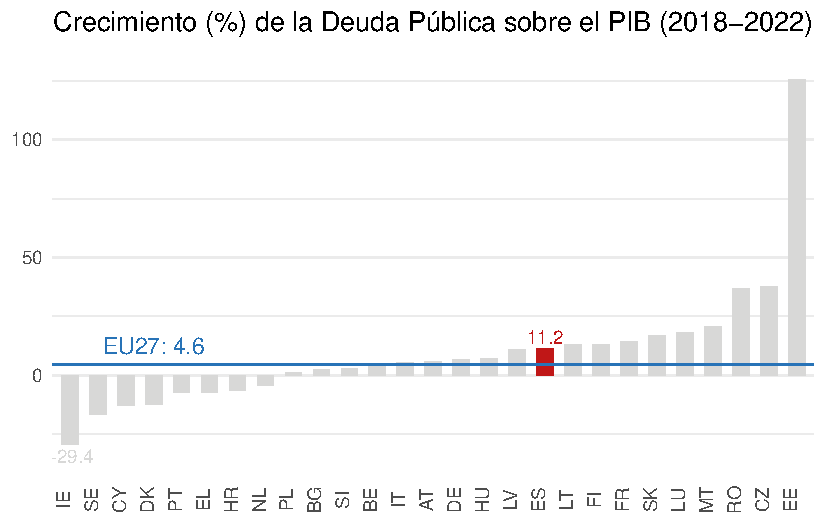
\includegraphics{Trabajo_files/figure-pdf/unnamed-chunk-31-1.pdf}

\hypertarget{resultados}{%
\section{Resultados}\label{resultados}}

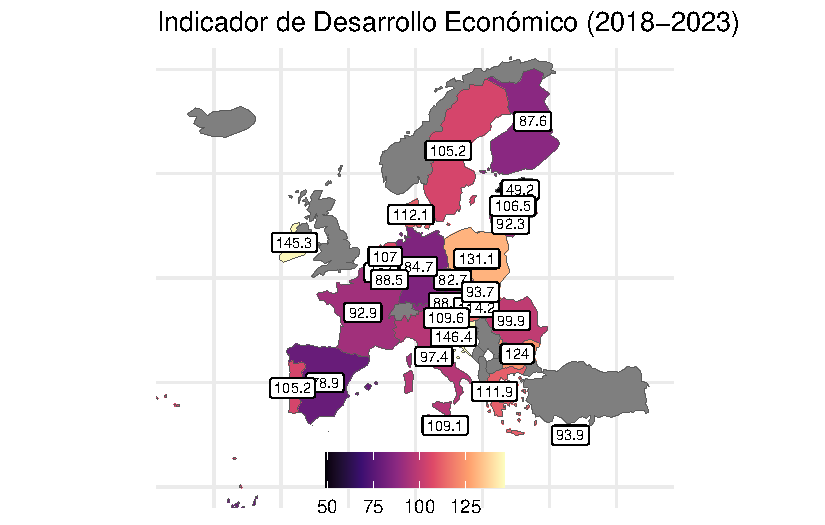
\includegraphics{Trabajo_files/figure-pdf/unnamed-chunk-36-1.pdf}

\hypertarget{conclusiones}{%
\section{Conclusiones}\label{conclusiones}}



\end{document}
